\section{Design}
	
%Based on the functional modules of LuCI, we will design the functional components of the Android application, which are organized into three major categories:
	
%\begin{itemize}
		
%		\item
%		\textbf{Network configuration} covers common functionalities in configuration tools that often come with commercial APs. These configurations include, but may not be limited to, managing network interfaces, DHCP and DNS settings, static routes, and firewall.
		
%		\item
%		\textbf{System configuration} provides an interface to customize the OpenWRT box. Common adminstration functions include: system and user configuration (setting device adminstrator password, creating system backup image and restoring system from backup image, generating user SSH keys, etc), software management (installing and configuring software packages) and task management (managing scheduled task and startup task). If the time allows, an in-application command line tool can be implemented for advanced users to execute console commands from the application to further customize the OpenWRT box.
		
%		\item
%		\textbf{Status/Statistics visualization} offers a mobile-phone friendly view of the system status (firmware and kernel version, uptime, current time; CPU and memory usage, currently running processes, system and kernel log) and network-related status (interface, route, firewall status, etc). The visualization component can provide real-time graphs of system load and traffic statistics, such as historical system memory usage, network traffic per interface and traffic per transport layer connection.
		
%\end{itemize}
	
%	The design and implementation effort will be organized by the three function categories, with approximately one and a half weeks dedicated to each.

\subsection{Backend}

\subsubsection{Application specific traffic statistics}
\label{sec:app-specific-design}

One of the goals in this project was to identify and provide statistics for traffic belonging to specific user applications, such as quantifying incoming and outgoing traffic related to specific smartphone application and services, and determining the identities of the hosts generating the traffic going through the OpenWRT box. To achieve this goal, we considered the two following design approaches:

\textbf{(A).} Pre-install a service on each user device that would monitor application network usage information from the operating system and report the monitored statistics to a service on the OpenWRT box. This approach can likely generate very accurate results and provide each specific application's statistical network usage. However, the major drawback to this method of collecting accurate traffic information is that it requires that each user voluntarily install and run this service on their devices, a requirement non-ideal for our goal: this service should not require additional actions and permissions from user devices, and the OpenWRT box should be able to collect statistics with or without end user cooperation.
	
\textbf{(B).}  Capture the traffic on the OpenWRT box, and run per-packet analysis. While less accurate than the first option, it is less intrusive to the user. The following information components from packet headers or payloads could be used to capture traffic:
	
	\begin{itemize}
		
		\item Source and destination IP addresses. 
		
		Popular service providers, such as Google and Facebook, own large chunks of IP addresses, and certain destination IP address ranges may correspond to servers for a specific application. By collecting such information and building a  mapping from destination IP address to an application's backend services, it is possible to infer which user application generated the traffic. The problem with this approach is that this mapping takes time to build, and dynamically changing the mapping in response to newly collected information is difficult, especially considering the fact that many popular services are using CDNs.
		
		\item Source and destination port number. 
		
		Certain services can be identified by IANA's port number allocation \cite{PortAssignment}, and this information is easily retrievable from the Internet. The problem with this approach is that the number of applications that can be identified purely by port number is very limited, as some applications will share the same ports. For example, the Youtube and Facebook apps on Android both go through port 443 (TLS).
		
		\item Application layer payload. 
		
		Decoding application payload and trying to find characteristic plain text is another way to identify which application a packet belongs to. This approach is promising, except it works only if such characteristic texts can be located and the application payload has not encrypted, which is not the case for most popular Android applications, such as Youtube or Facebook. Packet capturing of these Android applications shows that their traffic goes on top of TLS, and packet capturing of the activity of watching Youtube videos on a desktop indicates that the traffic goes on top of QUIC, which has encryption over UDP.
		
		\item Source and destination host names. 
		
		DNS host names often give information about the service provider, even when the service provider's using CDNs. By doing a DNS reverse lookup on the IP addresses, we can find out the service's domain name, thus infer what application's generating the traffic. The assumption behind this approach is that most servers or CDN boxes have a DNS name that corresponds to the application backend that they run. Our initial experiments suggest that this assumption is indeed true for popular applications like Youtube and Facebook, though mapping a DNS domain to a certain service may not be straightforward. For example, Facebook app on Android talks to both \textit{*.facebook.com} domain, and \textit{*.fbcdn.net} (owned by the CDN provider, Akamai Technologies) domain, and Youtube app talks to both \textit{*.google.com}, and \textit{*.1e100.net}, another Google owned domain. 
		
		Given this caveat, the authors chose the last approach since it is most applicable than other options listed above. For the proof-of-concept implementation, the mapping from domain names to service names is statically configured. It is also worth mentioning that this approach will limit our statistics to per service provider, rather than per exact application (for example, the traffic application is unable to differentiate Google Hangout application traffic from Youtube application traffic), but the authors believe this approach is enough for the purpose of providing statistics on the router end that provides a network adminstrator a reasonable amount of information to determine which applications on which devices are generating how much traffic.
		
	\end{itemize} 

\subsection{Mobile Application}
This sub-section describes the design of the OpenWRT remote access mobile application. Since this is a proof of concept, we only designed and implemented the application on Android platform.

\subsubsection{Architecture}
Figure \ref{android-architecture} shows the architecture of the Android OpenWRT remote access mobile application. It mainly contains four sub modules: activity module, network communication module, graphical user interfac module and response result parer module. Among these four modules, activities combine the other three modules together to present result to users and take users' inputs.
	\begin{figure*}
		\centering
		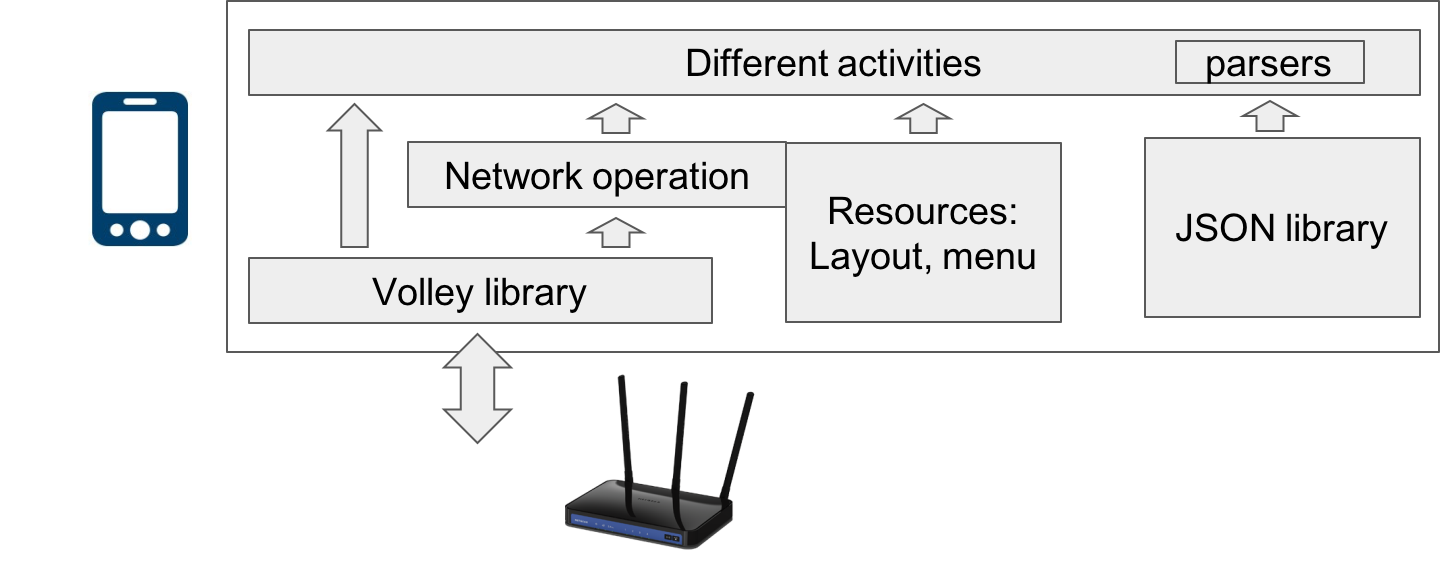
\includegraphics[width=0.75\textwidth]{android-architecture.png}
		\caption{Android Application Architecture}
		\label{android-architecture}
	\end{figure*}

\subsubsection{Network Communication}
Since the application needs to communicate with OpenWRT backend server, it's necessary to provide a network communication module to handle all the network operation, so that other modules can simply use its APIs without worrying about the details.

LuCI backend and application specific traffic analysis backend both provide http-based interfaces. To commuicate with these two backends, the network communication module needs to be able to send ``http POST'' and ``http GET'' requests and receives responses. A key part is to build proper URLs according to backends' requirments. The only difference between ``http POST'' and ``http GET'' is that ``http POST'' carries some parameters in the URL. For example, a ``http POST'' request to communicate with LuCI backend is ``http://<IP address of the OpenWrt Box>:<server port>/cgi-bin/luci/;stok=<stok id>''; a ``http GET'' request to communicate with application specific traffic analysis backend is ``http://<IP address of the OpenWrt Box>:<server port>/output.txt''

\subsubsection{Graphical User Interface}
The goal of the graphical user interface design was to simplify the user interface on a smartphone. To that end, the limitations of the LuCI web interface were studied to provide design guidelines. The first issue analyzed was that LuCI had an issue in its navigation on smartphones. To navigate through the application categories, the user needed to select a category in the navigation menu, then select a subcategory from the dropdown menu. Additionally, changing subcategories within the same category still required selecting the overarching category again. Therefore, a design goal of the application would be to maintain the current category and simply swap subcategories.
	
Another LuCI WebView issue was that unsaved changes would be tracked in a session until committed. Tracking unsaved changes on a web browser can result in session complications, depending on browser settings for caching. Furthermore, the WebView relied on in-browser scripting to provide functional elements, which is a dependency that can be optimized. Therefore another aspect of our design was to make all actions atomic and contained to the screen they are accessed on, to avoid carrying changes. To make all actions atomic, all functional elements in the original WebView would be rebuilt natively in Android.
	
Based on the LuCI framework, the designed Android application's user interface screens consisted of a login screen, then three major categories: status, network, and system. Each category then presented a subnavigation menu that persisted until another major category was selected, allowing users to move more freely within same category.
	
Each separate screen in the subcategories of the major categories was designed to maintain discrete actions and information. Rather than having multiple configuration forms and submission buttons in the same screen, the screen would be limited to at most one form each, with other forms being accessible on a new screen that is linked to by a list on the current screen.
